\documentclass[a4paper, 11pt]{article}
\usepackage[left=2cm,text={17cm, 24cm},top=3cm]{geometry}
\usepackage[utf8]{inputenc}
\usepackage[czech]{babel}
\usepackage{times}
\usepackage{multirow}
\usepackage[linesnumbered, ruled, lined]{algorithm2e}
\usepackage{graphicx}
\usepackage{epstopdf}
\usepackage{lscape}
\newcommand{\czuv}[1]{\quotedblbase #1\textquotedblleft}
\begin{document}
%%%%%%%%%%%%%%%%%%%%%%%FRONTPAGE%%%%%%%%%%%%%%%%%%%%%%%%%%%%%%%%%%%%
\thispagestyle{empty}
\begin{center}

\textsc{
\Huge{Vysoké učení technické v~Brně \\}
\huge{Fakulta informačních technologií\\}
}
\vspace{\stretch{0.382}}


\LARGE{Typografie a publikování -- 3. projekt \\}
\Huge{Tabulky a obrázky\\}
\vspace{\stretch{0.618}}

\end{center}

\Large{\today} \hfill Jiří Matějka

%%%%%%%%%%%%%%%%%%%%%%%%%%%%%%%%%%%%%%%%%%%%%%%%%%%%%%%%%%%%%%%%%%%%%%
\newpage
\normalsize
\setcounter{page}{1}
\section{Úvodní strana}
Název práce umístěte do zlatého řezu a nezapomeňte uvést dnešní datum a vaše jméno a příjmení.

%%%%%%%%%%%%%%%%%%%%%%%%%%%%%%%%%%%%%%%%%%%%%%%%%%%%%%%%%%%%%%%%%%%%%%%

\section{Tabulky}
Pro sázení tabulek můžeme použít buď prostředí \texttt{tabbing} nebo prostředí \texttt{tabular}.

\subsection{Prostředí \texttt{tabbing}}
Při použití \texttt{tabbing} vypadá tabulka následovně:
    \begin{tabbing}
    Vodní melouny \quad \= Cena \quad
    \= Množství \kill
    \bfseries Ovoce \>
    \bfseries Cena \>
    \bfseries Množství \\
    Jablka \> 25,90 \> 3 kg \\
    Hrušky \> 27,40 \>  2,5 kg \\
    Vodní melouny \> 35,-- \> 1 kus
    \end{tabbing}
Toto prostředí se dá také použít pro sázení algoritmů, ovšem vhodnější je použít 
prostředí \texttt{algorithm} nebo \texttt{algorithm2e} (viz sekce 3).

\subsection{Prostředí \texttt{tabular}}
Další možností, jak vytvořit tabulku, je použít prostředí \texttt{tabular}. Tabulky pak 
budou vypadat takto\footnote{Kdyby byl problém s \texttt{cline}, zkuste se podívat třeba sem:
http://www.abclinuxu.cz/tex/poradna/show/325037.}:
\begin{table}[h]
\centering
\begin{tabular}{|l|l|l|}
\hline
\textbf{}     & \multicolumn{2}{c|}{\textbf{Cena}} \\ \cline{2-3} 
\textbf{Měna} & \textbf{nákup}  & \textbf{prodej}  \\ \hline
EUR           & 27,34           & 27,42            \\
GBP           & 33,09           & 33,21            \\
USD           & 19,87           & 19,95            \\ \hline
\end{tabular}
\caption{Tabulka kurzů k dnešnímu dni}
\label{tab1}
\end{table}

\begin{table}[h]
\centering
\begin{tabular}{|l|l|}
\hline
A          & $\neg$A                      \\ \hline
\textbf{P} & N                      \\ \hline
\textbf{O} & O                      \\ \hline
\textbf{X} & X                      \\ \hline
\textbf{N} & P                      \\ \hline
\end{tabular}
\begin{tabular}{|l|l|l|l|l|l|}
\hline
\multicolumn{2}{|c|}{\multirow{2}{*}{$A \wedge B$}} & \multicolumn{4}{c|}{$B$}                            \\ \cline{3-6} 
\multicolumn{2}{|c|}{}                       & \textbf{P} & \textbf{O} & \textbf{X} & \textbf{N} \\ \hline
\multirow{4}{*}{$A$}        & \textbf{P}       & P          & O          & X          & N          \\ \cline{2-6} 
                          & \textbf{O}       & O          & O          & N          & N          \\ \cline{2-6} 
                          & \textbf{X}       & X          & N          & X          & N          \\ \cline{2-6} 
                          & \textbf{N}       & N          & N          & N          & N          \\ \hline
\end{tabular}
\begin{tabular}{|l|l|l|l|l|l|}
\hline
\multicolumn{2}{|c|}{\multirow{2}{*}{$A \vee B$}} & \multicolumn{4}{c|}{$B$}                            \\ \cline{3-6} 
\multicolumn{2}{|c|}{}                       & \textbf{P} & \textbf{O} & \textbf{X} & \textbf{N} \\ \hline
\multirow{4}{*}{$A$}        & \textbf{P}       & P          & P          & P          & P          \\ \cline{2-6} 
                          & \textbf{O}       & P          & O          & P          & O          \\ \cline{2-6} 
                          & \textbf{X}       & P          & P          & X          & X          \\ \cline{2-6} 
                          & \textbf{N}       & P          & O          & X          & N          \\ \hline
\end{tabular}
\begin{tabular}{|l|l|l|l|l|l|}
\hline
\multicolumn{2}{|c|}{\multirow{2}{*}{$A \rightarrow B$}} & \multicolumn{4}{c|}{$B$}                            \\ \cline{3-6} 
\multicolumn{2}{|c|}{}                       & \textbf{P} & \textbf{O} & \textbf{X} & \textbf{N} \\ \hline
\multirow{4}{*}{$A$}        & \textbf{P}       & P          & O          & X          & N          \\ \cline{2-6} 
                          & \textbf{O}       & P          & O          & P          & O          \\ \cline{2-6} 
                          & \textbf{X}       & P          & P          & X          & X          \\ \cline{2-6} 
                          & \textbf{N}       & P          & P          & P          & P          \\ \hline
\end{tabular}
\caption{Protože Kleeneho trojhodnotová logika už je \czuv{zastaralá}, uvádíme si zde příklad
čtyřhodnotové logiky}
\label{tab2}
\end{table}
\pagebreak
%%%%%%%%%%%%%%%%%%%%%%%%%%%%%%%%%%END_PAGE_1%%%%%%%%%%%%%%%%%%%%%%%%%%%%%

\section{Algoritmy}
Pokud budeme chtít vysázet algoritmus, můžeme použít prostředí
\texttt{algorithm\footnote{Pro nápovědu, jak zacházet s prostředím \texttt{algorithm}, můžeme zkusit tuhle stránku:
\\http://ftp.cstug.cz/pub/tex/CTAN/macros/latex/contrib/algorithms/algorithms.pdf.}}
nebo
\texttt{algorithm2e\footnote{Pro \texttt{algorithm2e} zase tuhle:
http://ftp.cstug.cz/pub/tex/CTAN/macros/latex/contrib/algorithm2e/doc/algorithm2e.pdf.}}.
Příklad použití prostředí \texttt{algorithm2e} viz Algoritmus 1.\\[0.5cm]

\begin{algorithm}[H]
\caption{\textsc{Fast}SLAM}
\label{alg1}
\SetKwInput{Input}{Input}
\SetKwInOut{Output}{Output}
\SetNlSty{}{}{:  }
\Input{$(X_{t-1},u_t,z_t)$}
\Output{$X_t$}
\BlankLine
\SetAlgoNoLine
\SetKwBlock{Beginn}{beginn}{ende}
$\overline{X_t} = X_t = 0$\\
\For{$k=1$ \normalfont{to} $M$} {
$x_t^{[k]} =$ \emph{sample\_motion\_model}$(u_t,x_{t-1}^{[k]})$\\
$w_t^{[k]} =$ \emph{measurement\_model}$(z_t,x_t^{[k]},m_{t-1})$\\
$m_t^{[k]} = updated\_occupancy\_grid(z_t,x_t^{[k]},m_{t-1}^{[k]})$\\
$\overline{X_t} = \overline{X_t} + \langle x_x^{[m]},w_t^{[m]}\rangle$
}
\For{$k=1$ \normalfont{to} $M$} {
draw $i$ with probability $\approx w_t^{[i]}$\\
add $\langle x_x^{[k]},m_t^{[k]}\rangle$ to $X_t$\\
}
\Return{$X_t$}
\end{algorithm}

%%%%%%%%%%%%%%%%%%%%%%%%%%%%%%%%%%%%%%%%%%%%%%%%%%%%%%%%%%%%%%%%%%%%%%%%%%
\section{Obrázky}
Do našich článků můžeme samozřejmě vkládat obrázky. Pokud je obrázkem fotografie,
můžeme klidně použít bitmapový soubor. Pokud by to ale mělo být nějaké schéma nebo
něco podobného, je dobrým zvykem takovýto obrázek vytvořit vektorově.

\begin{figure}[h]
\begin{center}
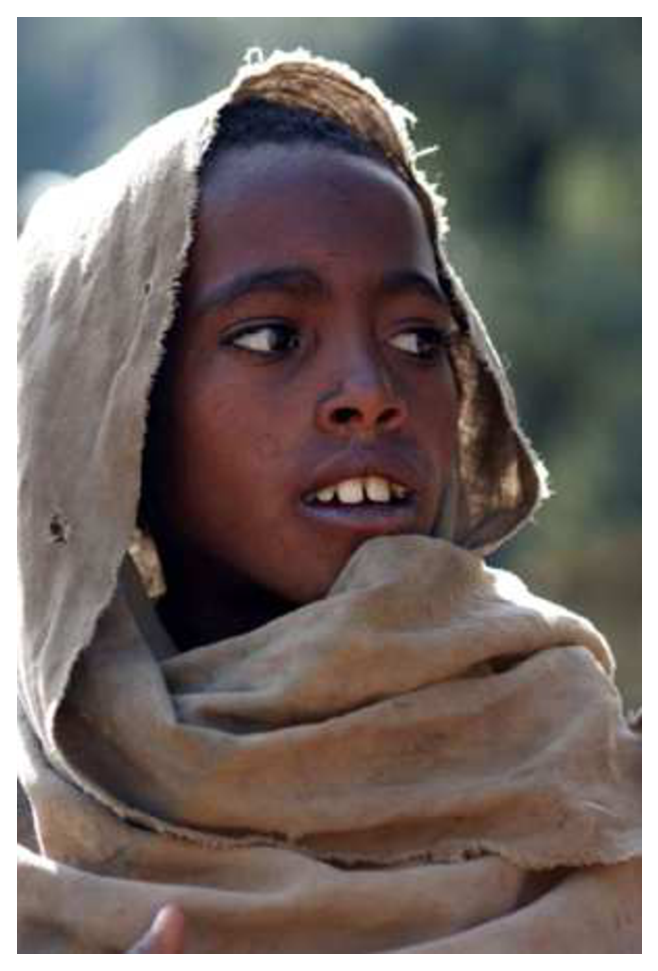
\includegraphics[scale=0.4]{etiopan.eps}
\reflectbox{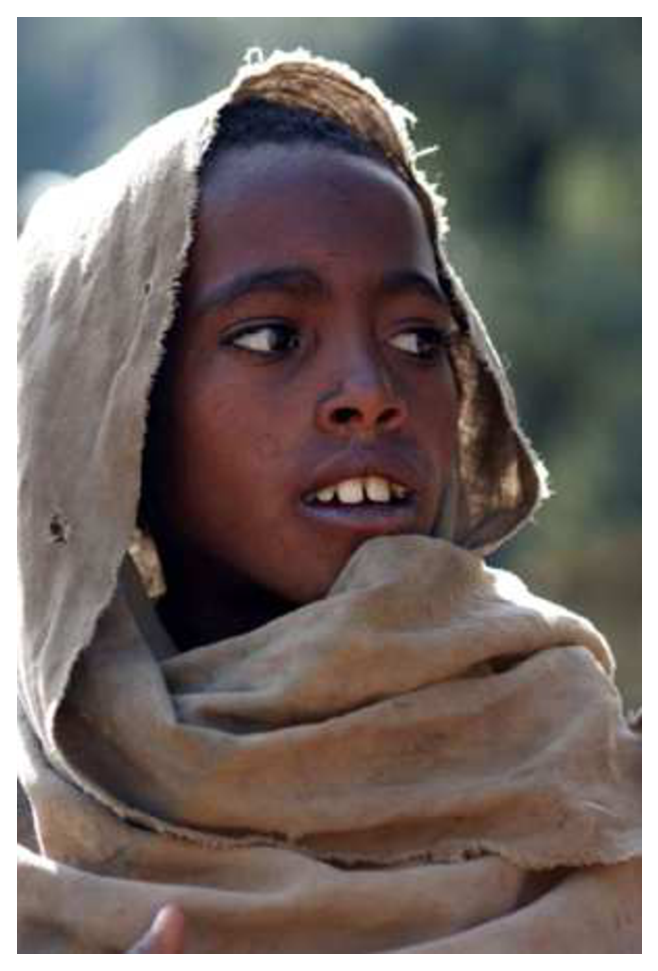
\includegraphics[scale=0.4]{etiopan.eps}}
\caption{Obrázek 1: Malý Etiopánek a jeho bratříček}
\label{im1}
\end{center}
\end{figure}
%%%%%%%%%%%%%%%%%%%%%%%%%%%%%%%%END_PAGE_2%%%%%%%%%%%%%%%%%%%%%%%%%%%%%%%%%%%%%


Rozdíl mezi vektorovým \ldots


\begin{figure}[h]	
\begin{center} 

\includegraphics[scale=0.4]{oniisan.eps} 
\caption{Vektorový obrázek}
\label{im2}
\end{center}
\end{figure}


\ldots a bitmapovým obrázkem


\begin{figure}[h]
\begin{center} 

\includegraphics[scale=0.6]{oniisan2.eps} 
\caption{Bitmapový obrázek}
\label{im3}
\end{center}
\end{figure}
Odkazy (nejen ty) na obrázky \ref{im1}, \ref{im2} a \ref{im3}, na  
tabulky \ref{tab1} a \ref{tab2} a také na algoritmus \ref{alg1} jsou udělány pomocí 
křížových odkazů. Pak je ovšem potřeba zdrojový soubor přeložit dvakrát.


Vektorové obrázky lze vytvořit i přímo v \LaTeX u, například pomocí prostředí 
\texttt{picture}.
\newpage
%%%%%%%%%%%%%%%%%%%%%%%%%%%%%%%%%%%%%%%%%%%%%%%%%%%%%%%%%%%%%%%%%%%%%%%%%%%%%%%%%
\begin{landscape}
TODO
\begin{figure}[h]
\begin{picture}(6,4)
%\put(0,0){\includesvg{kresba.svg}}
\end{picture}   
\end{figure}
\end{landscape}
\end{document}

